\documentclass{standalone}
\usepackage{tikz}
\usetikzlibrary{patterns, positioning}


\begin{document}
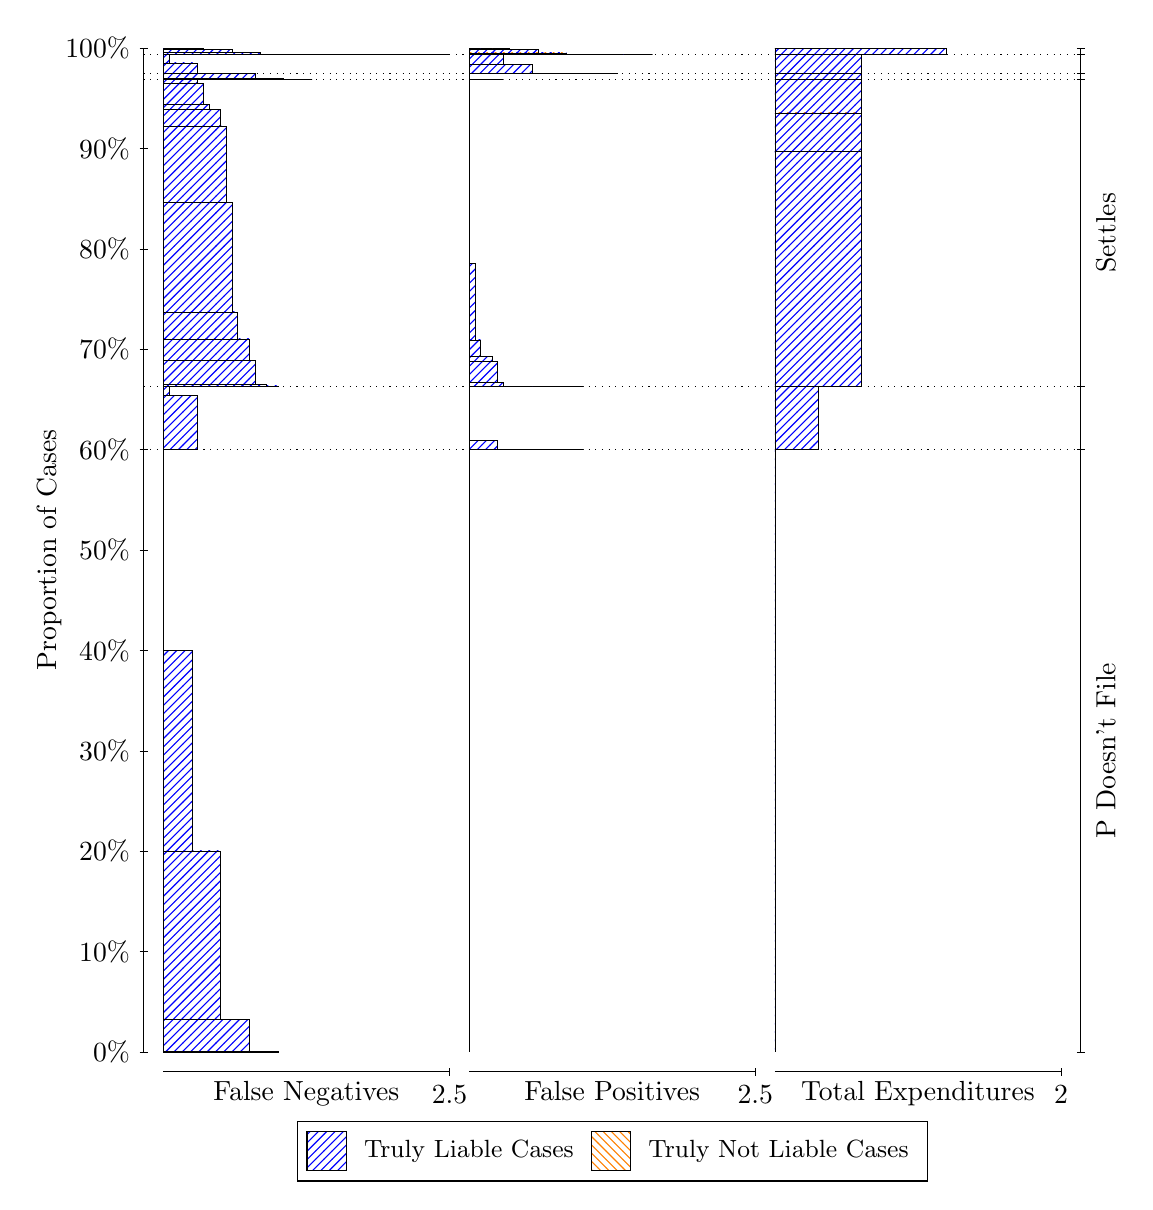
\begin{tikzpicture}
\draw[black, very thin] (1.5,1.75) -- (1.5,14.5);
\node[rotate=90, text=black, anchor=center] at (0.3, 8.125) {Proportion of Cases};
\draw[black, very thin] (1.45,1.75) -- (1.55,1.75);
\node[text=black, anchor=east] at (1.45, 1.75) {0\%};
\draw[black, very thin] (1.45,3.025) -- (1.55,3.025);
\node[text=black, anchor=east] at (1.45, 3.025) {10\%};
\draw[black, very thin] (1.45,4.3) -- (1.55,4.3);
\node[text=black, anchor=east] at (1.45, 4.3) {20\%};
\draw[black, very thin] (1.45,5.575) -- (1.55,5.575);
\node[text=black, anchor=east] at (1.45, 5.575) {30\%};
\draw[black, very thin] (1.45,6.85) -- (1.55,6.85);
\node[text=black, anchor=east] at (1.45, 6.85) {40\%};
\draw[black, very thin] (1.45,8.125) -- (1.55,8.125);
\node[text=black, anchor=east] at (1.45, 8.125) {50\%};
\draw[black, very thin] (1.45,9.4) -- (1.55,9.4);
\node[text=black, anchor=east] at (1.45, 9.4) {60\%};
\draw[black, very thin] (1.45,10.675) -- (1.55,10.675);
\node[text=black, anchor=east] at (1.45, 10.675) {70\%};
\draw[black, very thin] (1.45,11.95) -- (1.55,11.95);
\node[text=black, anchor=east] at (1.45, 11.95) {80\%};
\draw[black, very thin] (1.45,13.225) -- (1.55,13.225);
\node[text=black, anchor=east] at (1.45, 13.225) {90\%};
\draw[black, very thin] (1.45,14.5) -- (1.55,14.5);
\node[text=black, anchor=east] at (1.45, 14.5) {100\%};

\draw[black, very thin] (13.4,1.75) -- (13.4,14.5);
\draw[black, very thin] (13.35,1.75) -- (13.45,1.75);
\node[anchor=west] at (13.35, 1.75) {};
\draw[black, very thin] (13.35,9.4013) -- (13.45,9.4013);
\node[anchor=west] at (13.35, 9.4013) {};
\draw[black, very thin] (13.35,10.203) -- (13.45,10.203);
\node[anchor=west] at (13.35, 10.203) {};
\draw[black, very thin] (13.35,14.101) -- (13.45,14.101);
\node[anchor=west] at (13.35, 14.101) {};
\draw[black, very thin] (13.35,14.181) -- (13.45,14.181);
\node[anchor=west] at (13.35, 14.181) {};
\draw[black, very thin] (13.35,14.42) -- (13.45,14.42);
\node[anchor=west] at (13.35, 14.42) {};
\draw[black, very thin] (13.35,14.5) -- (13.45,14.5);
\node[anchor=west] at (13.35, 14.5) {};

\draw[black, very thin, pattern color=blue, pattern=north east lines] (1.75,1.75) rectangle (3.2033,1.7541);
\draw[black, very thin, pattern color=blue, pattern=north east lines] (1.75,1.7541) rectangle (2.84,2.1592);
\draw[black, very thin, pattern color=blue, pattern=north east lines] (1.75,2.1592) rectangle (2.4767,4.3047);
\draw[black, very thin, pattern color=blue, pattern=north east lines] (1.75,4.3047) rectangle (2.1133,6.8513);
\draw[black, very thin, pattern color=orange, pattern=north west lines] (1.75,6.8513) rectangle (1.75,6.8513);
\draw[black, very thin, pattern color=blue, pattern=north east lines] (1.75,6.8513) rectangle (1.75,9.4013);
\draw[black, very thin, pattern color=blue, pattern=north east lines] (1.75,9.4013) rectangle (2.186,10.09);
\draw[black, very thin, pattern color=blue, pattern=north east lines] (1.75,10.09) rectangle (1.8227,10.202);
\draw[black, very thin, pattern color=orange, pattern=north west lines] (1.75,10.202) rectangle (1.75,10.202);
\draw[black, very thin, pattern color=blue, pattern=north east lines] (1.75,10.202) rectangle (1.75,10.203);
\draw[black, very thin, pattern color=blue, pattern=north east lines] (1.75,10.203) rectangle (3.2033,10.208);
\draw[black, very thin, pattern color=blue, pattern=north east lines] (1.75,10.208) rectangle (3.058,10.23);
\draw[black, very thin, pattern color=blue, pattern=north east lines] (1.75,10.23) rectangle (2.9127,10.536);
\draw[black, very thin, pattern color=blue, pattern=north east lines] (1.75,10.536) rectangle (2.84,10.807);
\draw[black, very thin, pattern color=blue, pattern=north east lines] (1.75,10.807) rectangle (2.6947,11.148);
\draw[black, very thin, pattern color=blue, pattern=north east lines] (1.75,11.148) rectangle (2.622,12.539);
\draw[black, very thin, pattern color=blue, pattern=north east lines] (1.75,12.539) rectangle (2.5493,13.51);
\draw[black, very thin, pattern color=blue, pattern=north east lines] (1.75,13.51) rectangle (2.4767,13.723);
\draw[black, very thin, pattern color=blue, pattern=north east lines] (1.75,13.723) rectangle (2.3313,13.784);
\draw[black, very thin, pattern color=blue, pattern=north east lines] (1.75,13.784) rectangle (2.2587,14.052);
\draw[black, very thin, pattern color=blue, pattern=north east lines] (1.75,14.052) rectangle (2.186,14.098);
\draw[black, very thin, pattern color=blue, pattern=north east lines] (1.75,14.098) rectangle (2.1133,14.099);
\draw[black, very thin, pattern color=blue, pattern=north east lines] (1.75,14.099) rectangle (1.968,14.099);
\draw[black, very thin, pattern color=blue, pattern=north east lines] (1.75,14.099) rectangle (1.8953,14.101);
\draw[black, very thin, pattern color=blue, pattern=north east lines] (1.75,14.101) rectangle (1.8227,14.101);
\draw[black, very thin, pattern color=orange, pattern=north west lines] (1.75,14.101) rectangle (1.75,14.101);
\draw[black, very thin, pattern color=blue, pattern=north east lines] (1.75,14.101) rectangle (1.75,14.101);
\draw[black, very thin, pattern color=blue, pattern=north east lines] (1.75,14.101) rectangle (3.6393,14.101);
\draw[black, very thin, pattern color=blue, pattern=north east lines] (1.75,14.101) rectangle (3.276,14.114);
\draw[black, very thin, pattern color=blue, pattern=north east lines] (1.75,14.114) rectangle (2.9127,14.179);
\draw[black, very thin, pattern color=blue, pattern=north east lines] (1.75,14.179) rectangle (2.5493,14.181);
\draw[black, very thin, pattern color=blue, pattern=north east lines] (1.75,14.181) rectangle (2.186,14.181);
\draw[black, very thin, pattern color=orange, pattern=north west lines] (1.75,14.181) rectangle (1.75,14.181);
\draw[black, very thin, pattern color=blue, pattern=north east lines] (1.75,14.181) rectangle (2.186,14.311);
\draw[black, very thin, pattern color=blue, pattern=north east lines] (1.75,14.311) rectangle (1.8227,14.419);
\draw[black, very thin, pattern color=orange, pattern=north west lines] (1.75,14.419) rectangle (1.75,14.419);
\draw[black, very thin, pattern color=blue, pattern=north east lines] (1.75,14.419) rectangle (1.75,14.42);
\draw[black, very thin, pattern color=blue, pattern=north east lines] (1.75,14.42) rectangle (5.3833,14.42);
\draw[black, very thin, pattern color=blue, pattern=north east lines] (1.75,14.42) rectangle (5.02,14.42);
\draw[black, very thin, pattern color=blue, pattern=north east lines] (1.75,14.42) rectangle (4.6567,14.422);
\draw[black, very thin, pattern color=blue, pattern=north east lines] (1.75,14.422) rectangle (4.2933,14.424);
\draw[black, very thin, pattern color=blue, pattern=north east lines] (1.75,14.424) rectangle (3.93,14.424);
\draw[black, very thin, pattern color=blue, pattern=north east lines] (1.75,14.424) rectangle (3.712,14.424);
\draw[black, very thin, pattern color=blue, pattern=north east lines] (1.75,14.424) rectangle (3.5667,14.424);
\draw[black, very thin, pattern color=blue, pattern=north east lines] (1.75,14.424) rectangle (3.3487,14.424);
\draw[black, very thin, pattern color=blue, pattern=north east lines] (1.75,14.424) rectangle (3.2033,14.424);
\draw[black, very thin, pattern color=blue, pattern=north east lines] (1.75,14.424) rectangle (2.9853,14.441);
\draw[black, very thin, pattern color=blue, pattern=north east lines] (1.75,14.441) rectangle (2.622,14.482);
\draw[black, very thin, pattern color=blue, pattern=north east lines] (1.75,14.482) rectangle (2.2587,14.5);
\draw[black, very thin, pattern color=blue, pattern=north east lines] (1.75,14.5) rectangle (1.8953,14.5);
\draw[black, very thin, pattern color=orange, pattern=north west lines] (1.75,14.5) rectangle (1.75,14.5);
\draw[black, very thin, pattern color=blue, pattern=north east lines] (1.75,14.5) rectangle (1.75,14.5);
\draw[black, very thin, pattern color=orange, pattern=north west lines] (5.6333,1.75) rectangle (5.6333,1.75);
\draw[black, very thin, pattern color=blue, pattern=north east lines] (5.6333,1.75) rectangle (5.6333,9.4013);
\draw[black, very thin, pattern color=orange, pattern=north west lines] (5.6333,9.4013) rectangle (7.0867,9.4013);
\draw[black, very thin, pattern color=blue, pattern=north east lines] (5.6333,9.4013) rectangle (7.0867,9.4013);
\draw[black, very thin, pattern color=blue, pattern=north east lines] (5.6333,9.4013) rectangle (6.7233,9.4013);
\draw[black, very thin, pattern color=blue, pattern=north east lines] (5.6333,9.4013) rectangle (6.36,9.4015);
\draw[black, very thin, pattern color=blue, pattern=north east lines] (5.6333,9.4015) rectangle (5.9967,9.5141);
\draw[black, very thin, pattern color=blue, pattern=north east lines] (5.6333,9.5141) rectangle (5.6333,10.203);
\draw[black, very thin, pattern color=orange, pattern=north west lines] (5.6333,10.203) rectangle (7.0867,10.203);
\draw[black, very thin, pattern color=blue, pattern=north east lines] (5.6333,10.203) rectangle (7.0867,10.203);
\draw[black, very thin, pattern color=orange, pattern=north west lines] (5.6333,10.203) rectangle (6.796,10.203);
\draw[black, very thin, pattern color=blue, pattern=north east lines] (5.6333,10.203) rectangle (6.796,10.203);
\draw[black, very thin, pattern color=blue, pattern=north east lines] (5.6333,10.203) rectangle (6.7233,10.203);
\draw[black, very thin, pattern color=orange, pattern=north west lines] (5.6333,10.203) rectangle (6.6507,10.203);
\draw[black, very thin, pattern color=blue, pattern=north east lines] (5.6333,10.203) rectangle (6.6507,10.203);
\draw[black, very thin, pattern color=orange, pattern=north west lines] (5.6333,10.203) rectangle (6.5053,10.203);
\draw[black, very thin, pattern color=blue, pattern=north east lines] (5.6333,10.203) rectangle (6.5053,10.203);
\draw[black, very thin, pattern color=blue, pattern=north east lines] (5.6333,10.203) rectangle (6.4327,10.203);
\draw[black, very thin, pattern color=blue, pattern=north east lines] (5.6333,10.203) rectangle (6.36,10.205);
\draw[black, very thin, pattern color=blue, pattern=north east lines] (5.6333,10.205) rectangle (6.2873,10.205);
\draw[black, very thin, pattern color=blue, pattern=north east lines] (5.6333,10.205) rectangle (6.142,10.205);
\draw[black, very thin, pattern color=blue, pattern=north east lines] (5.6333,10.205) rectangle (6.0693,10.252);
\draw[black, very thin, pattern color=blue, pattern=north east lines] (5.6333,10.252) rectangle (5.9967,10.52);
\draw[black, very thin, pattern color=blue, pattern=north east lines] (5.6333,10.52) rectangle (5.924,10.581);
\draw[black, very thin, pattern color=blue, pattern=north east lines] (5.6333,10.581) rectangle (5.7787,10.794);
\draw[black, very thin, pattern color=blue, pattern=north east lines] (5.6333,10.794) rectangle (5.706,11.765);
\draw[black, very thin, pattern color=blue, pattern=north east lines] (5.6333,11.765) rectangle (5.6333,14.101);
\draw[black, very thin, pattern color=orange, pattern=north west lines] (5.6333,14.101) rectangle (6.0693,14.101);
\draw[black, very thin, pattern color=blue, pattern=north east lines] (5.6333,14.101) rectangle (6.0693,14.101);
\draw[black, very thin, pattern color=blue, pattern=north east lines] (5.6333,14.101) rectangle (5.706,14.104);
\draw[black, very thin, pattern color=blue, pattern=north east lines] (5.6333,14.104) rectangle (5.6333,14.181);
\draw[black, very thin, pattern color=orange, pattern=north west lines] (5.6333,14.181) rectangle (7.5227,14.181);
\draw[black, very thin, pattern color=blue, pattern=north east lines] (5.6333,14.181) rectangle (7.5227,14.181);
\draw[black, very thin, pattern color=blue, pattern=north east lines] (5.6333,14.181) rectangle (7.1593,14.181);
\draw[black, very thin, pattern color=blue, pattern=north east lines] (5.6333,14.181) rectangle (6.796,14.182);
\draw[black, very thin, pattern color=blue, pattern=north east lines] (5.6333,14.182) rectangle (6.4327,14.29);
\draw[black, very thin, pattern color=blue, pattern=north east lines] (5.6333,14.29) rectangle (6.0693,14.42);
\draw[black, very thin, pattern color=orange, pattern=north west lines] (5.6333,14.42) rectangle (7.9587,14.42);
\draw[black, very thin, pattern color=blue, pattern=north east lines] (5.6333,14.42) rectangle (7.9587,14.42);
\draw[black, very thin, pattern color=orange, pattern=north west lines] (5.6333,14.42) rectangle (7.5953,14.42);
\draw[black, very thin, pattern color=blue, pattern=north east lines] (5.6333,14.42) rectangle (7.5953,14.42);
\draw[black, very thin, pattern color=orange, pattern=north west lines] (5.6333,14.42) rectangle (7.232,14.42);
\draw[black, very thin, pattern color=blue, pattern=north east lines] (5.6333,14.42) rectangle (7.232,14.42);
\draw[black, very thin, pattern color=blue, pattern=north east lines] (5.6333,14.42) rectangle (6.8687,14.438);
\draw[black, very thin, pattern color=orange, pattern=north west lines] (5.6333,14.438) rectangle (6.8687,14.438);
\draw[black, very thin, pattern color=blue, pattern=north east lines] (5.6333,14.438) rectangle (6.8687,14.438);
\draw[black, very thin, pattern color=blue, pattern=north east lines] (5.6333,14.438) rectangle (6.5053,14.479);
\draw[black, very thin, pattern color=blue, pattern=north east lines] (5.6333,14.479) rectangle (6.5053,14.479);
\draw[black, very thin, pattern color=blue, pattern=north east lines] (5.6333,14.479) rectangle (6.142,14.493);
\draw[black, very thin, pattern color=blue, pattern=north east lines] (5.6333,14.493) rectangle (6.142,14.495);
\draw[black, very thin, pattern color=orange, pattern=north west lines] (5.6333,14.495) rectangle (5.924,14.495);
\draw[black, very thin, pattern color=blue, pattern=north east lines] (5.6333,14.495) rectangle (5.924,14.495);
\draw[black, very thin, pattern color=blue, pattern=north east lines] (5.6333,14.495) rectangle (5.7787,14.495);
\draw[black, very thin, pattern color=blue, pattern=north east lines] (5.6333,14.495) rectangle (5.7787,14.495);
\draw[black, very thin, pattern color=orange, pattern=north west lines] (5.6333,14.495) rectangle (5.6333,14.495);
\draw[black, very thin, pattern color=blue, pattern=north east lines] (5.6333,14.495) rectangle (5.6333,14.5);
\draw[black, very thin, pattern color=orange, pattern=north west lines] (9.5167,1.75) rectangle (9.5167,1.75);
\draw[black, very thin, pattern color=blue, pattern=north east lines] (9.5167,1.75) rectangle (9.5167,9.4013);
\draw[black, very thin, pattern color=orange, pattern=north west lines] (9.5167,9.4013) rectangle (10.062,9.4013);
\draw[black, very thin, pattern color=blue, pattern=north east lines] (9.5167,9.4013) rectangle (10.062,10.203);
\draw[black, very thin, pattern color=orange, pattern=north west lines] (9.5167,10.203) rectangle (10.607,10.203);
\draw[black, very thin, pattern color=blue, pattern=north east lines] (9.5167,10.203) rectangle (10.607,13.187);
\draw[black, very thin, pattern color=orange, pattern=north west lines] (9.5167,13.187) rectangle (10.607,13.187);
\draw[black, very thin, pattern color=blue, pattern=north east lines] (9.5167,13.187) rectangle (10.607,13.677);
\draw[black, very thin, pattern color=orange, pattern=north west lines] (9.5167,13.677) rectangle (10.607,13.677);
\draw[black, very thin, pattern color=blue, pattern=north east lines] (9.5167,13.677) rectangle (10.607,14.101);
\draw[black, very thin, pattern color=orange, pattern=north west lines] (9.5167,14.101) rectangle (10.607,14.101);
\draw[black, very thin, pattern color=blue, pattern=north east lines] (9.5167,14.101) rectangle (10.607,14.181);
\draw[black, very thin, pattern color=orange, pattern=north west lines] (9.5167,14.181) rectangle (10.607,14.181);
\draw[black, very thin, pattern color=blue, pattern=north east lines] (9.5167,14.181) rectangle (10.607,14.42);
\draw[black, very thin, pattern color=orange, pattern=north west lines] (9.5167,14.42) rectangle (11.697,14.42);
\draw[black, very thin, pattern color=blue, pattern=north east lines] (9.5167,14.42) rectangle (11.697,14.497);
\draw[black, very thin, pattern color=orange, pattern=north west lines] (9.5167,14.497) rectangle (11.697,14.497);
\draw[black, very thin, pattern color=blue, pattern=north east lines] (9.5167,14.497) rectangle (11.697,14.5);
\draw[black, dotted] (1.5,9.4013) -- (13.4,9.4013);
\draw[black, dotted] (1.5,10.203) -- (13.4,10.203);
\draw[black, dotted] (1.5,14.101) -- (13.4,14.101);
\draw[black, dotted] (1.5,14.181) -- (13.4,14.181);
\draw[black, dotted] (1.5,14.42) -- (13.4,14.42);
\draw[black, very thin] (1.75,1.5) -- (5.3833,1.5);
\node[text=black, anchor=north] at (3.5667, 1.5) {False Negatives};
\draw[black, very thin] (5.3833,1.45) -- (5.3833,1.55);
\node[text=black, anchor=north] at (5.3833, 1.45) {2.5};

\draw[black, very thin] (5.6333,1.5) -- (9.2667,1.5);
\node[text=black, anchor=north] at (7.45, 1.5) {False Positives};
\draw[black, very thin] (9.2667,1.45) -- (9.2667,1.55);
\node[text=black, anchor=north] at (9.2667, 1.45) {2.5};

\draw[black, very thin] (9.5167,1.5) -- (13.15,1.5);
\node[text=black, anchor=north] at (11.333, 1.5) {Total Expenditures};
\draw[black, very thin] (13.15,1.45) -- (13.15,1.55);
\node[text=black, anchor=north] at (13.15, 1.45) {2};

\node[text=black, centered, rotate=90] at (13.72, 5.5756) {P Doesn't File};

\node[text=black, centered, rotate=90] at (13.72, 12.152) {Settles};




\draw (7.449999999999999,1.5) node[draw=none] (baseCoordinate) {};
\begin{scope}[align=center]
        \matrix[scale=0.5, draw=black, below=0.5cm of baseCoordinate, nodes={draw}, column sep=0.1cm]{
            \node[rectangle, draw, minimum width=0.5cm, minimum height=0.5cm, pattern color=blue, pattern=north east lines] {}; &
            \node[draw=none, font=\small, text=black] (B) {Truly Liable Cases}; &
            \node[rectangle, draw, minimum width=0.5cm, minimum height=0.5cm, pattern color=orange, pattern=north west lines] {}; &
            \node[draw=none, font=\small, text=black] (B) {Truly Not Liable Cases}; \\
            };
\end{scope}

\end{tikzpicture}
\end{document}